\documentclass[11pt,a4paper]{article}

% ── Packages ──
\usepackage[utf8]{inputenc}
\usepackage[T1]{fontenc}
\usepackage{amsmath,amssymb,amsfonts}
\usepackage{booktabs}
\usepackage{graphicx}
\usepackage{hyperref}
\usepackage{geometry}
\usepackage{listings}
\usepackage{xcolor}
\usepackage{tikz}
\usetikzlibrary{arrows.meta,positioning,calc,fit}
\usepackage{algorithm}
\usepackage{algorithmic}
\usepackage{enumitem}
\usepackage{caption}

\geometry{margin=2.5cm}

% ── Code listing style ──
\definecolor{codebg}{RGB}{245,245,245}
\definecolor{codegreen}{RGB}{0,128,0}
\definecolor{codegray}{RGB}{128,128,128}
\definecolor{codepurple}{RGB}{128,0,128}

\lstdefinestyle{pythonstyle}{
    backgroundcolor=\color{codebg},
    commentstyle=\color{codegreen},
    keywordstyle=\color{blue},
    stringstyle=\color{codepurple},
    basicstyle=\ttfamily\small,
    breaklines=true,
    frame=single,
    rulecolor=\color{codegray},
    numbers=left,
    numberstyle=\tiny\color{codegray},
    tabsize=4,
    language=Python,
    showstringspaces=false,
}
\lstset{style=pythonstyle}

% ── Title ──
\title{\textbf{Embedding Extraction Mechanism}\\[0.3em]
\large TSFM-Graph Adapter --- TimesFM 2.5 200M}
\author{Zehra Sagin}
\date{March 2026}

\begin{document}
\maketitle
\tableofcontents
\newpage

%==========================================================================
\section{Architectural Context}
%==========================================================================

The TSFM-Graph Adapter employs a \textbf{two-branch architecture}. The embedding extraction mechanism operates exclusively within \textbf{Branch~A (Temporal)}, producing frozen patch-level representations that serve as the temporal query in the cross-attention fusion stage.

\begin{table}[h]
\centering
\caption{Two-branch architecture overview.}
\smallskip
\small
\resizebox{\textwidth}{!}{%
\begin{tabular}{@{}lllll@{}}
\toprule
\textbf{Branch} & \textbf{Input} & \textbf{Module} & \textbf{Output} & \textbf{Usage} \\
\midrule
A --- Temporal (frozen) & CO1 price series $(T,)$ & TimesFM 2.5 200M & $E_{\text{target}} \in \mathbb{R}^{P \times D}$ & Cross-Attention \textbf{Q} \\
B --- Graph (trainable) & 10 asset price history & NodeFeatureBuilder $\to$ GNN & $H \in \mathbb{R}^{N \times D}$ & Cross-Attention \textbf{KV} \\
\bottomrule
\end{tabular}%
}
\end{table}

\noindent
\textbf{Key constraint:} The TimesFM embedding \emph{never} enters the GNN. It is used \emph{only} as the temporal query $Q$ in cross-attention fusion.

\begin{itemize}[nosep]
    \item $N = 10$ (number of commodity assets)
    \item $P = 32$ (number of patches = $1024 / 32$)
    \item $D = 1280$ (TimesFM model dimension)
    \item Patch length $p = 32$
    \item Max context $= 1024$
\end{itemize}

%==========================================================================
\section{TimesFMEmbeddingExtractor}
%==========================================================================

\texttt{TimesFMEmbeddingExtractor} accesses the \emph{internal layers} of the frozen TimesFM backbone to convert a raw price time series into patch-level embeddings. All computation runs under \texttt{torch.no\_grad()} --- no gradients flow through the backbone.

\subsection{End-to-End Pipeline}

For a single asset (\texttt{extract\_single}):

\[
\underbrace{(T,)}_{\text{raw series}}
\xrightarrow{\text{Pad/Trunc}}
\underbrace{(1024,)}_{\text{fixed length}}
\xrightarrow{\text{Patch}}
\underbrace{(32, 32)}_{\text{P patches}}
\xrightarrow{\text{RevIN}}
\underbrace{(32, 32)}_{\text{normalized}}
\xrightarrow{\text{TimesFM}}
\underbrace{(32, 1280)}_{\text{embeddings}}
\]

%--------------------------------------------------------------------------
\subsection{Step 1 --- Input Preparation (Pad + Mask)}
%--------------------------------------------------------------------------

Given a time series $\mathbf{x} \in \mathbb{R}^T$:

\begin{itemize}[nosep]
    \item If $T \geq 1024$: take the last 1024 values; mask $= \mathbf{0}$ (all real).
    \item If $T < 1024$: left-pad with zeros; mask $= [\underbrace{1,\ldots,1}_{\text{pad}},\underbrace{0,\ldots,0}_{T}]$.
\end{itemize}

\noindent
The mask convention: $\text{mask}[i] = 1$ means ``this value is padding (not real data).''

\begin{lstlisting}
if len(ts) >= max_context:
    value = ts[-max_context:]         # last 1024 values
    mask  = np.zeros(1024, bool)      # all real
else:
    pad_len = 1024 - len(ts)
    value = np.pad(ts, (pad_len, 0))  # left-pad with zeros
    mask  = [True]*pad_len + [False]*len(ts)
\end{lstlisting}

%--------------------------------------------------------------------------
\subsection{Step 2 --- Patching}
%--------------------------------------------------------------------------

The padded 1024-length vector is reshaped into $P = 32$ non-overlapping patches of length $p = 32$:

\[
\mathbf{v} \in \mathbb{R}^{1024} \;\longrightarrow\; \mathbf{X}_{\text{patched}} \in \mathbb{R}^{32 \times 32}
\]

\begin{lstlisting}
patched_inputs = inputs.reshape(N, 32, 32)  # (1, 32, 32)
patched_masks  = masks.reshape(N, 32, 32)
\end{lstlisting}

\noindent
Each patch covers 32 consecutive days:

\begin{center}
\begin{tabular}{@{}ll@{}}
\toprule
\textbf{Patch} & \textbf{Days} \\
\midrule
Patch 0    & Day 1--32 \\
Patch 1    & Day 33--64 \\
$\vdots$   & $\vdots$ \\
Patch 31   & Day 993--1024 \\
\bottomrule
\end{tabular}
\end{center}

%--------------------------------------------------------------------------
\subsection{Step 3 --- RevIN Running Statistics (Welford's Algorithm)}
%--------------------------------------------------------------------------

TimesFM uses \textbf{Reversible Instance Normalization (RevIN)} with causally accumulated statistics. Each patch is normalized using the running mean and standard deviation computed from \emph{all patches up to and including itself} --- no future information leaks.

\subsubsection{Per-Patch Incremental Statistics}

For patch $i$ with values $\{x_{i,j}\}$ and validity mask $\text{is\_legit}_{i,j} = \neg\text{mask}_{i,j}$:

\begin{align}
n_{\text{inc}} &= \sum_{j=1}^{p} \mathbb{1}[\text{is\_legit}_{i,j}] \label{eq:inc_n} \\[4pt]
\mu_{\text{inc}} &= \frac{1}{n_{\text{inc}}} \sum_{j=1}^{p} x_{i,j} \cdot \mathbb{1}[\text{is\_legit}_{i,j}] \label{eq:inc_mu} \\[4pt]
\sigma^2_{\text{inc}} &= \frac{1}{n_{\text{inc}}} \sum_{j=1}^{p} (x_{i,j} - \mu_{\text{inc}})^2 \cdot \mathbb{1}[\text{is\_legit}_{i,j}] \label{eq:inc_var}
\end{align}

\noindent
If $n_{\text{inc}} = 0$ (fully masked patch): $\mu_{\text{inc}} = 0,\; \sigma_{\text{inc}} = 0$.

\subsubsection{Cumulative Update (Welford's Parallel Merge)}

Let $(n, \mu, \sigma)$ be the cumulative statistics \emph{before} patch $i$, and $(n_{\text{inc}}, \mu_{\text{inc}}, \sigma_{\text{inc}})$ be the statistics of patch $i$. The updated cumulative statistics are:

\begin{align}
n_{\text{new}} &= n + n_{\text{inc}} \label{eq:new_n} \\[6pt]
\mu_{\text{new}} &= \frac{n \cdot \mu + n_{\text{inc}} \cdot \mu_{\text{inc}}}{n_{\text{new}}} \label{eq:new_mu} \\[6pt]
\sigma^2_{\text{new}} &= \frac{%
    n \cdot \sigma^2
    + n_{\text{inc}} \cdot \sigma^2_{\text{inc}}
    + n \cdot (\mu - \mu_{\text{new}})^2
    + n_{\text{inc}} \cdot (\mu_{\text{inc}} - \mu_{\text{new}})^2
}{n_{\text{new}}} \label{eq:new_var}
\end{align}

\noindent
This ensures that at patch $i$, the normalization uses statistics from days $1$ through $32(i+1)$ only --- \textbf{causal, no lookahead}.

\begin{center}
\begin{tabular}{@{}lll@{}}
\toprule
\textbf{Patch} & $\mu$ \textbf{computed from} & $\sigma$ \textbf{computed from} \\
\midrule
Patch 0 & Patch 0 only & Patch 0 only \\
Patch 1 & Patch 0 $+$ 1 & Patch 0 $+$ 1 \\
$\vdots$ & $\vdots$ & $\vdots$ \\
Patch 31 & All 32 patches & All 32 patches \\
\bottomrule
\end{tabular}
\end{center}

%--------------------------------------------------------------------------
\subsection{Step 4 --- RevIN Normalization}
%--------------------------------------------------------------------------

Each patch is normalized using its causally accumulated statistics:

\begin{equation}
\hat{x}_{i,j} = \frac{x_{i,j} - \mu_i}{\max(\sigma_i,\; \epsilon)}
\qquad \text{where } \epsilon = 10^{-6}
\label{eq:revin}
\end{equation}

Padded positions are zeroed out after normalization:
\[
\hat{x}_{i,j} \leftarrow
\begin{cases}
\hat{x}_{i,j} & \text{if } \text{is\_legit}_{i,j} = \text{True} \\
0 & \text{otherwise}
\end{cases}
\]

%--------------------------------------------------------------------------
\subsection{Step 5 --- TimesFM Forward Pass (Frozen)}
%--------------------------------------------------------------------------

The normalized patches $\hat{\mathbf{X}} \in \mathbb{R}^{32 \times 32}$ are fed through the frozen TimesFM backbone:

\[
\hat{\mathbf{X}} \in \mathbb{R}^{32 \times 32}
\;\xrightarrow{\text{Tokenizer}}\;
\mathbb{R}^{32 \times 64}
\;\xrightarrow{\text{Linear}}\;
\mathbb{R}^{32 \times 1280}
\;\xrightarrow{20\times \text{Transformer}}\;
\mathbf{E} \in \mathbb{R}^{32 \times 1280}
\]

\begin{lstlisting}
(_, output_emb, _, _), _ = self.module(normed_inputs, patched_masks, None)
# output_emb: (1, 32, 1280)
\end{lstlisting}

\noindent
The output $\mathbf{E} \in \mathbb{R}^{P \times D}$ contains one 1280-dimensional embedding per patch.

\textbf{No pooling is applied} --- all 32 patch embeddings are preserved. The last patch $\mathbf{E}[-1] \in \mathbb{R}^{1280}$ is later used by the prediction head.

%==========================================================================
\section{EmbeddingCache}
%==========================================================================

\subsection{Motivation}

Since the TimesFM backbone is \textbf{frozen}, identical inputs always produce identical outputs. Recomputing embeddings every epoch is wasteful:

\begin{table}[h]
\centering
\caption{Training speed comparison.}
\begin{tabular}{@{}lcc@{}}
\toprule
& \textbf{TimesFM per batch} & \textbf{Cached} \\
\midrule
Batch time & $\sim$1.75\,s & $\sim$0.01\,s \\
50 epochs total & $\sim$9 hours & $\sim$15 minutes \\
\bottomrule
\end{tabular}
\end{table}

\subsection{What It Stores}

Before training begins, the cache pre-computes \textbf{only the target asset's (CO1)} embedding for every sliding window position $t$:

\[
\forall\, t \in \text{positions}: \quad
\texttt{cache}[t] = \text{extract\_single}\!\bigl(\text{CO1}_{[t-1024:\,t]}\bigr) \in \mathbb{R}^{32 \times 1280}
\]

\begin{lstlisting}
for t in positions:
    context = all_data[max(0, t-1024):t]   # (<=1024, 10)
    target_series = context[:, 0]           # CO1 only
    seq_emb = extractor.extract_single(target_series, 1024)
    self.target_seq_cache[t] = seq_emb.cpu().numpy()  # (32, 1280)
\end{lstlisting}

\noindent
Only the target asset is cached --- the other 9 assets' embeddings are \emph{not needed} because the GNN uses handcrafted features exclusively. This yields \textbf{10$\times$ less memory} compared to caching all assets.

\subsection{Cache Retrieval During Training}

\begin{lstlisting}
# In commodity_graph_forecast.py:
target_seq = embedding_cache.get(pos, device)   # (32, 1280)
pred = model.forward_cached(
    target_seq_embeddings=target_seq,  # Cross-Attention Q
    price_history=price_hist,          # Graph branch input
)
\end{lstlisting}

\subsection{Persistence}

The cache supports disk serialization via \texttt{np.savez\_compressed}:
\begin{itemize}[nosep]
    \item \texttt{save(path)}: writes \texttt{seq\_keys} and \texttt{seq\_values} arrays.
    \item \texttt{load(path)}: restores the cache from disk, avoiding recomputation.
\end{itemize}

%==========================================================================
\section{Integration: \texttt{forward\_cached()}}
%==========================================================================

During training, \texttt{forward\_cached()} orchestrates the full pipeline \emph{without} running TimesFM:

\begin{figure}[h]
\centering
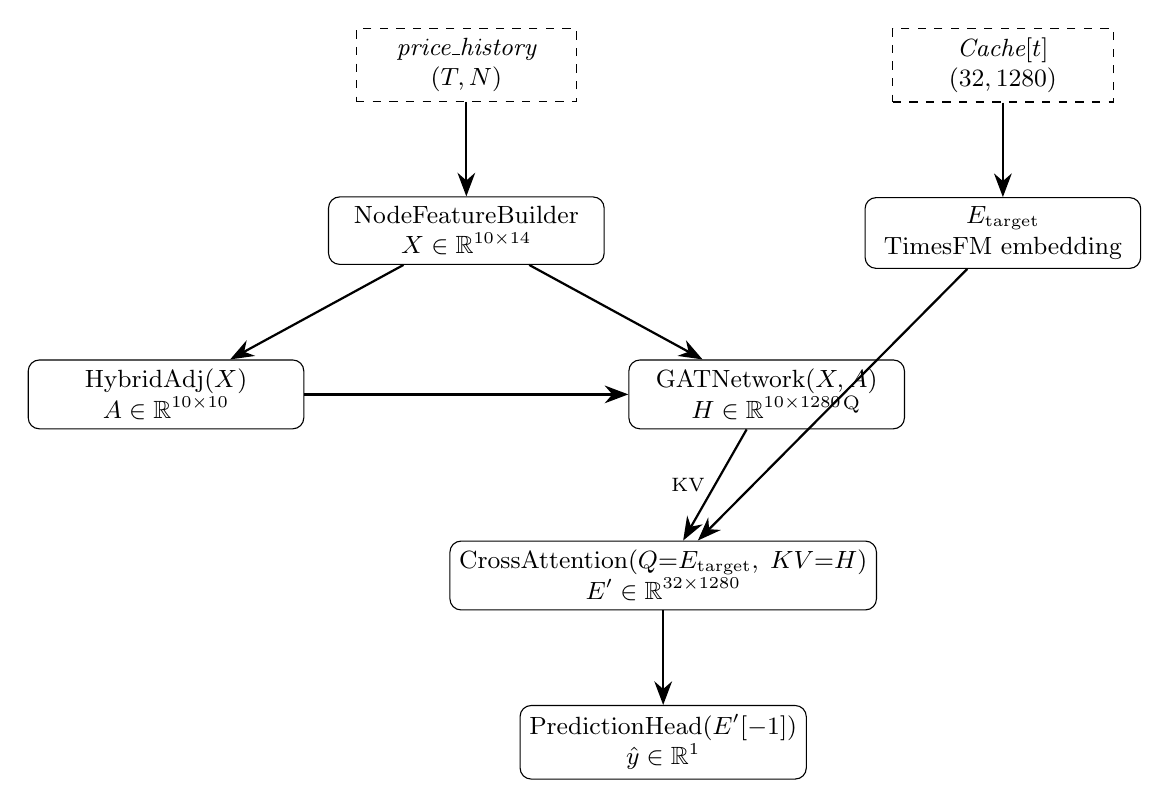
\begin{tikzpicture}[
    node distance=1.2cm and 2.5cm,
    block/.style={rectangle, draw, rounded corners, minimum width=3.5cm, minimum height=0.8cm, align=center, font=\small},
    data/.style={rectangle, draw, dashed, minimum width=2.8cm, minimum height=0.7cm, align=center, font=\small\itshape},
    arrow/.style={-{Stealth[length=3mm]}, thick},
]

% Left branch (Graph)
\node[data] (prices) {price\_history\\$(T, N)$};
\node[block, below=of prices] (nfb) {NodeFeatureBuilder\\$X \in \mathbb{R}^{10 \times 14}$};
\node[block, below left=1.2cm and 0.3cm of nfb] (adj) {HybridAdj$(X)$\\$A \in \mathbb{R}^{10 \times 10}$};
\node[block, below right=1.2cm and 0.3cm of nfb] (gat) {GATNetwork$(X, A)$\\$H \in \mathbb{R}^{10 \times 1280}$};

% Right branch (Cache)
\node[data, right=4cm of prices] (cache) {Cache$[t]$\\$(32, 1280)$};
\node[block, below=of cache] (emb) {$E_{\text{target}}$\\TimesFM embedding};

% Fusion
\node[block, below=3.5cm of nfb, xshift=2.5cm, minimum width=5cm] (fusion) {CrossAttention$(Q{=}E_{\text{target}},\; KV{=}H)$\\$E' \in \mathbb{R}^{32 \times 1280}$};

% Output
\node[block, below=of fusion] (head) {PredictionHead$(E'[-1])$\\$\hat{y} \in \mathbb{R}^{1}$};

% Arrows
\draw[arrow] (prices) -- (nfb);
\draw[arrow] (nfb) -- (adj);
\draw[arrow] (nfb) -- (gat);
\draw[arrow] (adj) -- (gat);
\draw[arrow] (gat) -- (fusion) node[midway, left, font=\scriptsize] {KV};
\draw[arrow] (cache) -- (emb);
\draw[arrow] (emb) -- (fusion) node[midway, right, font=\scriptsize] {Q};
\draw[arrow] (fusion) -- (head);

\end{tikzpicture}
\caption{Data flow in \texttt{forward\_cached()}. TimesFM does not run during training --- embeddings come from the pre-computed cache.}
\label{fig:forward_cached}
\end{figure}

\noindent
Step by step:

\begin{enumerate}[nosep]
    \item \textbf{Cache} $\to$ $E_{\text{target}} \in \mathbb{R}^{32 \times 1280}$: pre-computed TimesFM embedding (no forward pass).
    \item \textbf{NodeFeatureBuilder} $\to$ $X \in \mathbb{R}^{10 \times 14}$: handcrafted features from price history.
    \item \textbf{HybridGraphStructure}$(X)$ $\to$ $A \in \mathbb{R}^{10 \times 10}$: adjacency matrix (correlation $\cup$ sector $\cup$ supply chain $\cup$ learned).
    \item \textbf{GATNetwork}$(X, A)$ $\to$ $H \in \mathbb{R}^{10 \times 1280}$: cross-sectional graph context.
    \item \textbf{CrossAttention}$(Q{=}E_{\text{target}},\; KV{=}H)$ $\to$ $E' \in \mathbb{R}^{32 \times 1280}$: temporally enhanced embedding.
    \item \textbf{PredictionHead}$(E'[-1])$ $\to$ $\hat{y} \in \mathbb{R}^{1}$: delta price forecast.
\end{enumerate}

%==========================================================================
\section{Summary: The Embedding's Journey}
%==========================================================================

\begin{equation*}
\boxed{
\begin{aligned}
&\text{CO1 raw prices } (1024 \text{ days}) \\
&\quad \xrightarrow{\text{Pad/Truncate}} (1024,) \\
&\quad \xrightarrow{\text{Patch}} (32, 32) \\
&\quad \xrightarrow{\text{RevIN}} (32, 32) \text{ normalized} \\
&\quad \xrightarrow{\text{Tokenizer}} (32, 64) \to (32, 1280) \\
&\quad \xrightarrow{20\times\text{Transformer}} \mathbf{E} \in \mathbb{R}^{32 \times 1280} \quad \leftarrow \textbf{saved to cache} \\
&\quad \xrightarrow{\text{cache.get}(t)} E_{\text{target}} \in \mathbb{R}^{32 \times 1280} \\
&\quad \xrightarrow{\text{CrossAttn}(Q{=}E_{\text{target}},\; KV{=}H)} E' \in \mathbb{R}^{32 \times 1280} \\
&\quad \xrightarrow{\text{PredHead}(E'[-1])} \hat{y} \in \mathbb{R}^{1}
\end{aligned}
}
\end{equation*}

\end{document}
